%!TEX root = ../../report.tex
\chapter{Construction process} % (fold)
\label{cha:implementation}
This chapter is dedicated to explain the process of manufacturing and assembling the introduced designs.
From the important role of emerging low-cost technologies like FFF 3D printing up to the creation of custom PCBs for reducing the weight of the robot, the following sections are meant to explain the process of acquisition and construction of all the components of RuBi presented in previous chapters.
The implementation of the final prototype has always been led by criteria of security, constrained budget and feasibility for maintenance and futures improvements.

%!TEX root = ../../../report.tex
\section{3D printing} % (fold)
\label{sec:3d_printing}
The parts modeled for the project and shown in the section \ref{sub:computer_aided_design}, have been printed using Fused Filament Fabrication (FFF).
The 3D printer used is a M Prime One \footnote{https://github.com/M-Prime/M_Prime_One} with a 0.4 mm noozle.
All the parts have been printed at 0.2 mm layer height.

The use of this technology is justify by the fact that makes the iterative process between design and manufacturing both fast and cheap.
All the parts have been individually adjusted until the clearances have been as expected.
Furthermore, this enable the user not only to replicate the parts with out any considered extra cost, but allows the robot to be easily replicated in other places.

When manufacturing, some of the parts have needed material support.
The figure \ref{fig:photo_material_support} depicts two feet, one with material support and the other with it removed.
In the figure \ref{fig:photo_3d_printed} a detail of actual parts 3D printed and assembled in the robot are shown.

\begin{figure}[ht]
    \centering
    \begin{subfigure}[b]{0.49\textwidth}
        \includegraphics[width=\textwidth]{figures/photo_material_support.jpg}
        \caption{Feet with and without material support}
        \label{fig:photo_material_support}
    \end{subfigure}
    \begin{subfigure}[b]{0.49\textwidth}
        \includegraphics[width=\textwidth]{figures/photo_3d_printed.jpg}
        \caption{Detail of 3D printed parts assembled}
        \label{fig:photo_3d_printed}
    \end{subfigure}
\end{figure}

  \subsection{Arc compensation} % (fold)
  \label{sub:arc_compensation}
  For the CAD models of the 3D printed parts, the clearances of the internal holes have been adjusted following \cite{arc_compensation}.
  The undersizing of internal holes is a common problem in this sort of technology due to the lack of information of the common-used exporting format: the STL.
  This only contains the 3D model expressed as a set of external triangles, which difficult the correction of malformations inherent to the technology.

  In the case of the Fused Filament Fabrication (FFF), the material is extruded equally in both sides of the arc, as shown in \ref{fig:arc_compensation}. 
  However, in the side of the smaller curve, less material is needed.
  This correction can be calculated with:
  $$ r=\frac{t+\sqrt{t^2+4R^2}}{2}$$
  being:
  \begin{enumerate}
    \item t: noozle diameter
    \item R: desired internal hole radius
    \item r: corrected radius
  \end{enumerate}
  As an example, Klee suggests an internal hole of 4.4 mm in the case of the selected nuts \cite{klee}. Thus, the diameter in the CAD model has been adjusted for this data and a noozle of 0.4 mm. The result is then:
  $$ d=2r=\frac{t+\sqrt{t^2+4R^2}}{2}=0.4+\sqrt{0.4^2+4*2.2^2}=4.81$$

  \begin{figure}[tb]
    \centering
    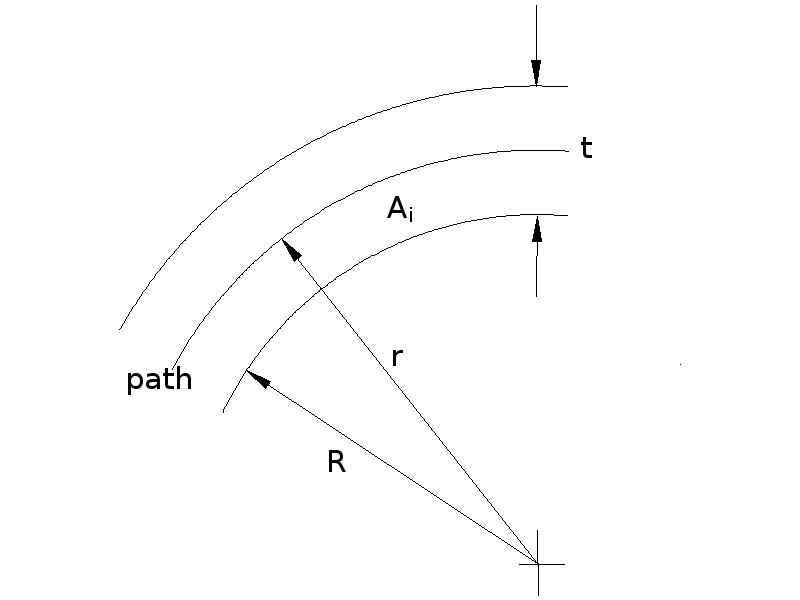
\includegraphics[width=0.5\textwidth]{figures/Arc-compensation}
    \caption{Technical representation of the generated arc when using FFF technology}
    \label{fig:arc_compensation}
  \end{figure}
  % subsection arc_compensation (end)

% section 3d_printing (end)
%!TEX root = ../../../report.tex
\section{Machining} % (fold)
\label{sec:machining}
Along with 3D printing, other parts have needed to be machined.
As an example, the rods came in bars of one meter that have been cut and filed according the design.
Other example are the carbon fiber tubes.
These have been designed to carry the wiring inside them.
Thus some holes have been performed in the bottom and top part of the tube in order to insert them.
The drawings for such parts are included as appendices in \ref{app:mechanical_drawings}.
% section machining (end)
%!TEX root = ../../../report.tex
\section{PCBs and wiring} % (fold)
\label{sec:pcbs_and_wiring}

% section pcbs_and_wiring (end)
%!TEX root = ../../../report.tex
\section{Providers} % (fold)
\label{sec:providers}
In addition to the 3D printed and machined parts, other items have been bought from several providers.
The providers have been selected based on previous shoppings made by the Mærsk Mc-Kinney Møller Institute.
All the needed items that could have followed an standard have been chosen. 
As an example, the robot only needs three types of screws (only M3 metric) and one kind of bearing.
The components are easily found and are not rare items or exotic materials that increase the price of the robot.
A list with all the components bought and its providers is attached as an appendix in \ref{app:order_list}.

As explained in the management of the project \ref{sec:project_management}, all the parts that are bought, included the springs, are ordered in the end of April. 
This was decided due to the delivery of the parts is a process that can take up to three weeks.
Despite all the parts where got within the first week, the springs have not been received, what has impeded the complete assembling of the robot.
However their fastening is easily made by following the assembly manuals provided and other experiments in which the springs are not needed will be carried out.

% section providers (end)
%!TEX root = ../../../report.tex
\section{Assembly} % (fold)
\label{sec:assembly}
Due to the fact that basically all the parts have been linked making use of 3D-printed parts, and all the tolerances of these have been adjusted individually, the assembly has been found easy and fast.
The mounting process has proved to be rapid enough to change some of the parts, as the springs, within minutes.
Furthermore, in the event of mechanical failure of any of the 3D-printed parts, its production and replacement is simple enough to reduce the maintenance time.
This result of employing 3D-printed parts can be considered as one of the main advantages of the whole platform.
The tension of the belts have been adjusted experimentally as explained in the section \ref{sub:pulleys_and_belts} using the zip ties installed.
In Figure \ref{fig:photo_robot_walking}, the complete robot assembled is shown while in \ref{fig:photo_dacbot}, a size comparison between the DACbot \cite{dacbot1} and RuBi can be done.

\begin{figure}[ht!]
    \centering
    \begin{subfigure}[b]{0.49\textwidth}
        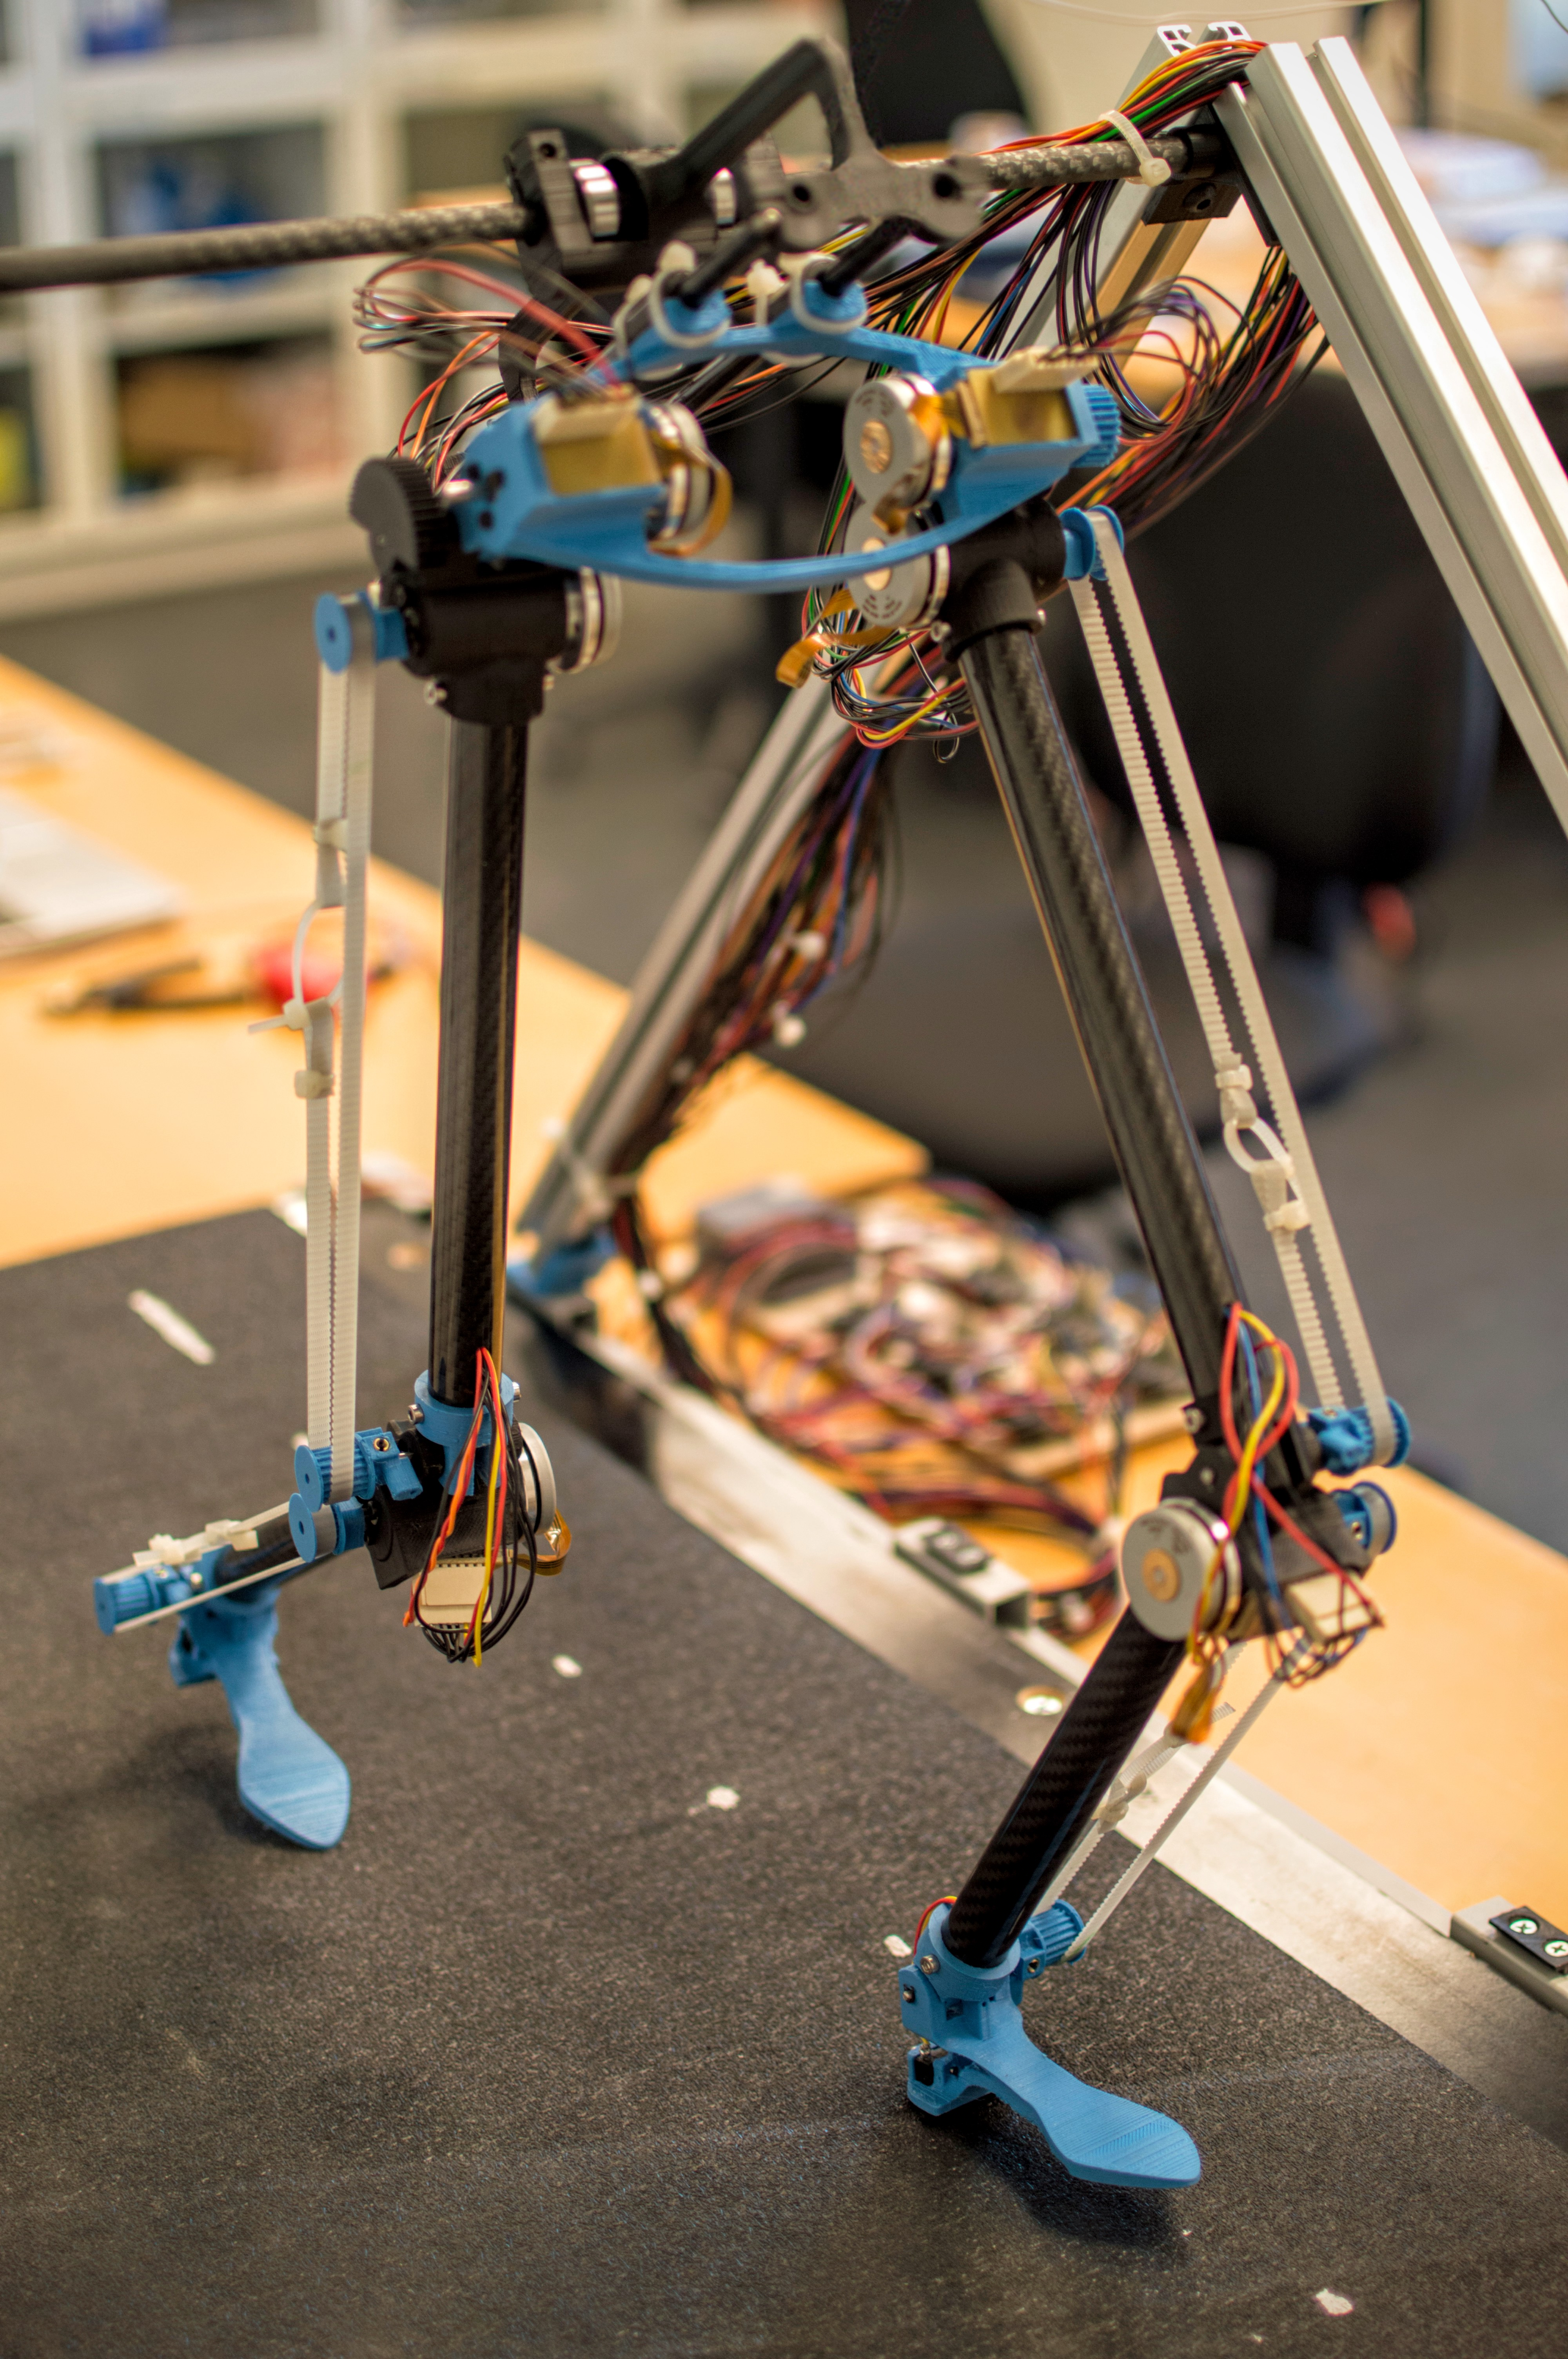
\includegraphics[width=\textwidth]{figures/photo_robot_walking.jpg}
        \caption{RuBi assembled.}
        \label{fig:photo_robot_walking}
    \end{subfigure}
    \begin{subfigure}[b]{0.49\textwidth}
        \includegraphics[width=\textwidth]{figures/photo_dacbot.jpg}
        \caption{RuBi and DACbot over the same treadmill.}
        \label{fig:photo_dacbot}
    \end{subfigure}
\end{figure}    
% section assembly (end)
%%!TEX root = ../../../report.tex
\section{How to bring up the robot} % (fold)
\label{sec:how_to_bring_up_the_robot}
In order to bring up the robot, a battery has to power it and the computer must be started.
It will automatically create a Wi-Fi hotspot called \textit{RuBi} where the user can connect to.
From this moment, the robot should be able to relocokit_hwceive motor commands.
If not, the IP in the \textit{locokit\_hw} has to be changed according to the stablished in the host.
In the guest, open a new terminal and run:

\begin{lstlisting}
roslaunch rubi_bringup rubi_bringup.launch
\end{lstlisting}

ROS Control will be loaded along with the locokit hardware interface and the controllers can move the real robot.
% section how_to_bring_up_the_robot (end)

% chapter implementation (end)